% -------------------------------
% Documento principal - Ingeniería en Sistemas
% -------------------------------
\documentclass[12pt, a4paper, oneside]{book}
\input{include/configuracion}

\begin{document}

% -------------------------------
% Plantilla del Anteproyecto en la Sede Regional Brunca. Versión 0.0 (Preliminar)
%
% CTFG Sede Regional Brunca
% 
% Compilar con XeLaTeX 
% -------------------------------
\pagestyle{empty}
\begin{titlepage}\null

\begin{textblock*}{\paperwidth}(0cm,4cm)
\begin{center}
\begin{figure}[ht]
    \centerline{
\includegraphics[scale=0.4]{figs/logo_una.jpg}}
\end{figure}
\end{center}
\end{textblock*}

\begin{textblock*}{\paperwidth}(0cm,9cm) 
\begin{center}\doublespacing
{\fontsize{16pt}{2pt}\selectfont Universidad Nacional de Costa Rica}

{\fontsize{16pt}{2pt}\selectfont Sede Regional Brunca}

{\fontsize{16pt}{2pt}\selectfont Campus PZ - Coto}
\end{center}
\end{textblock*}

\begin{textblock*}{\paperwidth}(0cm,13.5cm) 
\begin{center}\doublespacing 
{\bf\fontsize{18pt}{4pt}\selectfont Cátedra Ingeniería en Sistemas}

{\fontsize{16pt}{4pt}\selectfont Bachillerato en Ingeniería en Sistemas de Información}
\end{center}
\end{textblock*}

% --- Estudiantes ---
\begin{textblock*}{\paperwidth}(0cm,18cm) 
\begin{center}
{\Large\textbf{Estudiantes:}\par}
\vspace{0.5cm}
{\large Francisco Mora Cabezas\par}
{\large Ángel Segura Méndez\par}
\end{center}
\end{textblock*}

\begin{textblock*}{\paperwidth}(0cm,25.5cm) 
\begin{center}
% (Aquí podrías añadir fecha o lugar si lo piden)
\end{center}
\end{textblock*}

\end{titlepage}


\tableofcontents
\listoffigures
\listoftables

% --- Capítulos (no se tocan) ---

\chapter{Introducción} 

La Universidad Nacional de Costa Rica (UNA) busca modernizar y optimizar sus sistemas de gestión, especialmente aquellos relacionados con la calidad académica y la administración de recursos. En este contexto, la universidad enfrenta desafíos significativos en dos áreas clave: por un lado, la gestión de evidencias para los procesos de acreditación ante el Sistema Nacional de Acreditación de la Educación Superior (SINAES), y por otro, la administración eficiente de los tiempos de jornada universitaria, un recurso vital para la docencia y los proyectos institucionales.

Actualmente, la gestión de evidencias SINAES se realiza de manera manual y se apoya en una estructura de almacenamiento basada en carpetas en Google Drive. Este enfoque genera ineficiencias significativas, como la redundancia documental, una clasificación manual que consume un promedio de dos horas diarias por coordinador, y una marcada dificultad para correlacionar las evidencias con los criterios específicos de calidad definidos por SINAES. El problema principal radica en la ausencia de un sistema automatizado que permita una categorización eficiente y la falta de metadatos asociados a los documentos, lo que resulta en una dependencia de criterios individuales para la clasificación. Estas deficiencias no solo conllevan un desperdicio de recursos institucionales y la duplicación de la memoria utilizada, sino que también incrementan el riesgo de errores en la verificación del cumplimiento de criterios y pueden generar retrasos críticos en la preparación de informes para auditorías SINAES. Además, la falta de seguridad adecuada para los documentos institucionales representa un riesgo potencial de pérdida de acreditación en carreras clave. Para mitigar estos desafíos, se propone el desarrollo de un módulo de gestión de evidencias como parte del macro-proyecto "Gestión de Calidad", el cual estará enfocado exclusivamente en la interfaz de usuario para la manipulación directa de documentos en Google Drive, sin una capa de backend dedicada en esta fase inicial.
   % Introducción
\chapter{Antecedentes}

La Universidad Nacional (UNA) es una institución pública de educación superior costarricense, comprometida con la excelencia académica y la pertinencia social de sus programas formativos. Desde su fundación en 1973, la UNA ha impulsado procesos de evaluación y mejora continua con el propósito de garantizar la calidad de la educación superior en el país \cite{UNAweb}.

En el ámbito de la acreditación, la Universidad participa activamente en los procesos regulados por el Sistema Nacional de Acreditación de la Educación Superior (SINAES), organismo que establece estándares de calidad a partir de dimensiones, componentes y criterios específicos \cite{SINAES}. Este marco exige a las carreras universitarias disponer de mecanismos formales para recopilar, organizar y reportar evidencias que sustenten el cumplimiento de dichos criterios.

Asimismo, la UNA administra de forma permanente recursos humanos y académicos a través de los denominados tiempos de jornada, los cuales representan unidades de planificación y presupuesto destinadas a la asignación de labores docentes y de proyectos institucionales. La gestión de este recurso resulta estratégica para garantizar la equidad en la distribución de la carga académica y la ejecución eficiente de iniciativas de investigación y extensión.

La revisión de documentos institucionales y normativas evidencia la necesidad de fortalecer los procesos administrativos y académicos mediante herramientas tecnológicas que permitan centralizar, automatizar y resguardar la información relacionada con acreditación y planificación de tiempos de jornada \cite{ReglamentoUNA, InformeSINAES}.
   % Antecedentes 
\chapter{Descripción del Proyecto}

El proyecto se enmarca dentro del macro-proyecto denominado ``Gestión de Calidad'', cuyo propósito es apoyar a la Universidad Nacional en la optimización de procesos administrativos y académicos mediante la digitalización y automatización de la información clave. Este esfuerzo responde a la necesidad institucional de contar con sistemas más confiables, eficientes y seguros para la gestión de procesos vinculados con la acreditación académica y la distribución de recursos humanos y académicos.

De forma particular, se desarrollan dos módulos principales: 

\section*{Sistema de Gestión de Evidencias para Acreditación SINAES}

El Sistema de Gestión de Evidencias tiene como objetivo atender las debilidades actuales en la administración de documentos requeridos por los procesos de acreditación. Actualmente, la gestión se realiza mediante carpetas en Google Drive, lo que genera duplicidad, pérdida de tiempo en la búsqueda, falta de metadatos estandarizados y riesgo de inconsistencias en los informes.

El módulo propuesto introduce una estructura jerárquica de navegación (dimensión $\to$ componente $\to$ criterio) alineada con los lineamientos del SINAES, garantizando que cada evidencia se ubique en el criterio que le corresponde. Asimismo, cada documento se enriquece con metadatos normalizados (tipo, responsable, fecha, carrera, periodo), lo que permite búsquedas rápidas y generación de reportes confiables.

\subsection*{Funcionalidades principales}
\begin{itemize}
  \item Registro de evidencias con validación de formatos (PDF, DOCX, XLSX, PNG).
  \item Asignación de metadatos obligatorios y opcionales según el criterio SINAES.
  \item Búsqueda avanzada y filtrado por carrera, criterio, estado de cumplimiento o fecha.
  \item Generación de reportes en PDF con tablas comparativas por carrera o facultad.
  \item Registro de auditoría de accesos y modificaciones.
\end{itemize}

\subsection*{Beneficios esperados}
\begin{itemize}
  \item Reducción del tiempo de clasificación manual en al menos un 70\%.
  \item Mejora en la trazabilidad documental y en la preparación de auditorías.
  \item Aseguramiento de la integridad y centralización de los documentos institucionales.
  \item Disminución del riesgo de pérdida de acreditaciones por falta de evidencias confiables.
\end{itemize}

\subsection*{Alcances y limitaciones}
En esta primera fase, el sistema se concentrará en la interfaz de usuario y en la integración con Google Drive como repositorio oficial. No se incluye aún un backend propio para la gestión de evidencias, dado que el objetivo es entregar un prototipo funcional que demuestre la factibilidad y utilidad del modelo planteado.

\section*{Sistema de Gestión de Tiempos de Jornada Universitarios}

El Sistema de Tiempos de Jornada atiende la necesidad de distribuir de manera justa y transparente la carga docente y los recursos destinados a proyectos institucionales. Actualmente, la administración se realiza con hojas de cálculo que dificultan la consolidación de información, generan errores de cálculo y limitan la capacidad de generar reportes confiables.

Este módulo permitirá calcular automáticamente las horas de jornada según las mallas curriculares, los incrementos por repitencia y los tiempos otorgados por convenios externos. Además, se registrarán proyectos institucionales con consumo de tiempo docente, lo que aportará una visión integral de la utilización de este recurso.

\subsection*{Funcionalidades principales}
\begin{itemize}
  \item CRUD de catálogos (carreras, cursos, mallas curriculares, docentes y grupos).
  \item Registro y actualización de cargas docentes por periodo académico.
  \item Gestión de proyectos institucionales con asignación de horas.
  \item Reglas de cálculo para contemplar repitencia y tiempos externos (fijos e inciertos).
  \item Exportes de reportes en Excel por ciclo, carrera, sede y comparativos históricos.
\end{itemize}

\subsection*{Beneficios esperados}
\begin{itemize}
  \item Transparencia en la asignación de carga académica entre docentes.
  \item Optimización en el uso del presupuesto destinado a tiempos de jornada.
  \item Reducción de errores de cálculo por el uso de herramientas automatizadas.
  \item Base de datos centralizada que facilita la generación de reportes estratégicos.
\end{itemize}

\subsection*{Alcances y limitaciones}
El sistema se desarrollará con una base de datos no relacional en MongoDB, administrada a través de un backend en NestJS con Prisma ORM. En la presente etapa no se contempla la integración con otros sistemas de la universidad, aunque la arquitectura se diseñará modular para permitir futuras expansiones.

\bigskip

\noindent En conjunto, ambos módulos fortalecen la capacidad institucional de planificación estratégica, garantizando mayor eficiencia, transparencia y confiabilidad en la gestión académica y administrativa de la UNA. Además, constituyen un primer paso hacia la construcción de un ecosistema digital integral para la gestión de la calidad en la universidad.
   % Descripción del proyecto
\chapter{Planteamiento del Problema}

En la Universidad Nacional, los procesos de gestión de evidencias para la acreditación de carreras presentan dificultades asociadas con la dispersión, duplicidad y falta de trazabilidad de los documentos institucionales. Estas limitaciones provocan retrasos en la preparación de informes para los procesos de acreditación del SINAES y aumentan el riesgo de incumplimiento de los estándares de calidad exigidos.

De forma paralela, la administración de los tiempos de jornada universitarios se lleva a cabo mediante procedimientos manuales o apoyados en hojas de cálculo, lo cual genera inconsistencias en el cálculo de cargas docentes, dificultades en la planificación de proyectos institucionales y una limitada capacidad para generar reportes confiables en el corto plazo.

Esta situación refleja la ausencia de un mecanismo tecnológico unificado que permita centralizar y automatizar la gestión de evidencias y de tiempos de jornada. Dicha carencia afecta directamente la eficiencia administrativa, la transparencia en la toma de decisiones y la capacidad institucional para responder a los procesos de acreditación y planificación académica.

En consecuencia, se identifica como problema la necesidad de implementar un sistema web integrado que atienda estas deficiencias, facilite el cumplimiento de estándares de calidad y fortalezca la gestión estratégica de la Universidad Nacional.
   % Planteamiento del problema 
\chapter{Justificación}
\section{Justificación e importancia}
La implementación de estos sistemas es crucial para superar las limitaciones de los procesos manuales actuales en ambas áreas. Para la gestión de evidencias, se abordará la dificultad de acceso, organización y control, lo que se traducirá en:
\begin{itemize}
    \item Reducción significativa del tiempo de clasificación manual (hasta 70\% de ahorro).
    \item Eliminación de la duplicidad de archivos (abordando 35\% de discrepancias).
    \item Garantía del cumplimiento continuo de los estándares definidos por SINAES.
    \item Centralización efectiva de más de 500 documentos anuales con metadatos estructurados.
    \item Mejora de la seguridad y trazabilidad de la información sensible institucional.
\end{itemize}
Para el módulo de tiempos de jornada, el sistema representa una herramienta clave para la planificación eficiente de recursos humanos y académicos de la universidad, permitiendo tomar mejores decisiones sobre asignaciones docentes, ejecución de proyectos y administración del presupuesto anual de tiempos de jornada. La combinación de ambos módulos bajo el paraguas de "Gestión de Calidad" optimizará la toma de decisiones estratégicas y operativas en la UNA.
   % Justificación e importancia
\chapter{Objetivos}

Los objetivos definen los propósitos del trabajo y los límites de lo que se desea alcanzar con el desarrollo del proyecto. Se estructuran en un objetivo general y varios objetivos específicos, redactados en infinitivo y con criterios de verificación.

\section{Objetivo general}
Desarrollar un sistema web modular que automatice la gestión de evidencias SINAES y la administración de tiempos de jornada universitaria, mejorando la trazabilidad, la transparencia y la eficiencia operativa de la UNA mediante entregas incrementales alineadas al cronograma de sprints.

\section{Objetivos específicos}

\subsection*{Módulo Evidencias SINAES}
\begin{enumerate}
  \item Diseñar la interfaz jerárquica (dimensión $\rightarrow$ componente $\rightarrow$ criterio) para asociar evidencias SINAES, validada con al menos 3 casos de uso completos.
  \item Implementar el cargador de evidencias con metadatos obligatorios (tipo, responsable, fecha, carrera, período) y etiquetas; registrar al menos 20 evidencias de prueba.
  \item Generar reportes en PDF sobre estado de cumplimiento por carrera y facultad, incluyendo filtros por período y exportación descargable.
  \item Definir y aplicar un modelo de auditoría (altas, bajas, cambios, descargas) que conserve un historial mínimo de 30 días.
  \item Reducir el tiempo promedio de clasificación documental a \(\leq 30\) minutos por usuario mediante formularios guiados y metadatos estandarizados (prueba con 3 usuarios).
\end{enumerate}

\subsection*{Módulo Tiempos de Jornada}
\begin{enumerate}\setcounter{enumi}{5}
  \item Modelar el dominio académico de tiempos de jornada (carreras, mallas, cursos, grupos, docentes, reglas) en una base NoSQL documentada.
  \item Implementar los CRUD de cargas docentes y proyectos institucionales con validaciones de reglas de negocio.
  \item Incorporar el cálculo automático de repitencia y tiempos externos (fijos e inciertos), mostrando el detalle del cómputo por docente.
  \item Desarrollar exportes a Excel por ciclo, carrera y sede, con comparativos históricos (al menos dos períodos).
  \item Publicar un prototipo web funcional (frontend + API) con autenticación, documentación Swagger y evidencia de pruebas básicas (Smoke/Happy path).
\end{enumerate}
   % Objetivos
\chapter{Metodología}

\subsection{Fundamentación}
Para el desarrollo de los sistemas que conforman el macro-proyecto \textbf{“Gestión de Calidad”}, incluyendo el módulo de \textbf{gestión de evidencias} y el módulo de \textbf{gestión de tiempos de jornada}, se adoptó la metodología ágil \textbf{Scrum}.  

Esta decisión se basa en la necesidad de gestionar un proyecto modular y complejo, con requisitos que evolucionan en función de los procesos de acreditación universitaria (SINAES) y de la dinámica institucional.  

Las principales razones de su selección incluyen:
\begin{itemize}
    \item \textbf{Entregas incrementales}: se realizan entregas funcionales frecuentes a los diferentes stakeholders (Comité de Calidad SINAES, administración, docentes), permitiendo retroalimentación continua.
    \item \textbf{Flexibilidad y adaptabilidad}: Scrum facilita la incorporación de cambios en los criterios de acreditación y en las necesidades de los usuarios sin afectar la planificación global.
    \item \textbf{Alineación con el cronograma académico}: la iteración por sprints se ajusta a los semestres académicos y a los avances parciales solicitados en el curso.
    \item \textbf{Modularidad}: la arquitectura de los módulos permite construir bases funcionales mínimas y agregar nuevas características progresivamente.
\end{itemize}

\subsection{Referencia al WBS}
El marco metodológico se complementa con la \textbf{Estructura de Desglose del Trabajo (WBS)}, que organiza los entregables y actividades principales del proyecto en fases y módulos. El WBS fue elaborado en una herramienta formal (\emph{WBS Schedule Pro}), conforme a la observación docente, y sirve de guía para la planificación de sprints y la asignación de responsabilidades.

La Figura~\ref{fig:wbs} muestra la estructura jerárquica del proyecto y su correspondencia con los artefactos de Scrum:
\begin{itemize}
  \item \textbf{Nivel 1 (Proyecto):} alcance global del macro-proyecto \emph{Gestión de Calidad}.
  \item \textbf{Nivel 2 (Módulos/Fases):} Evidencias SINAES, Tiempos de Jornada, Integración/QA, Documentación/Estándares, Despliegue/Cierre.
  \item \textbf{Nivel 3 (Entregables):} análisis, diseño UI/UX, implementación (CRUDs, reportes), pruebas, documentación.
  \item \textbf{Nivel 4 (Paquetes de trabajo):} tareas planificables en sprints (vinculadas al \emph{Sprint Backlog}).
\end{itemize}

\begin{figure}[H]
  \centering
  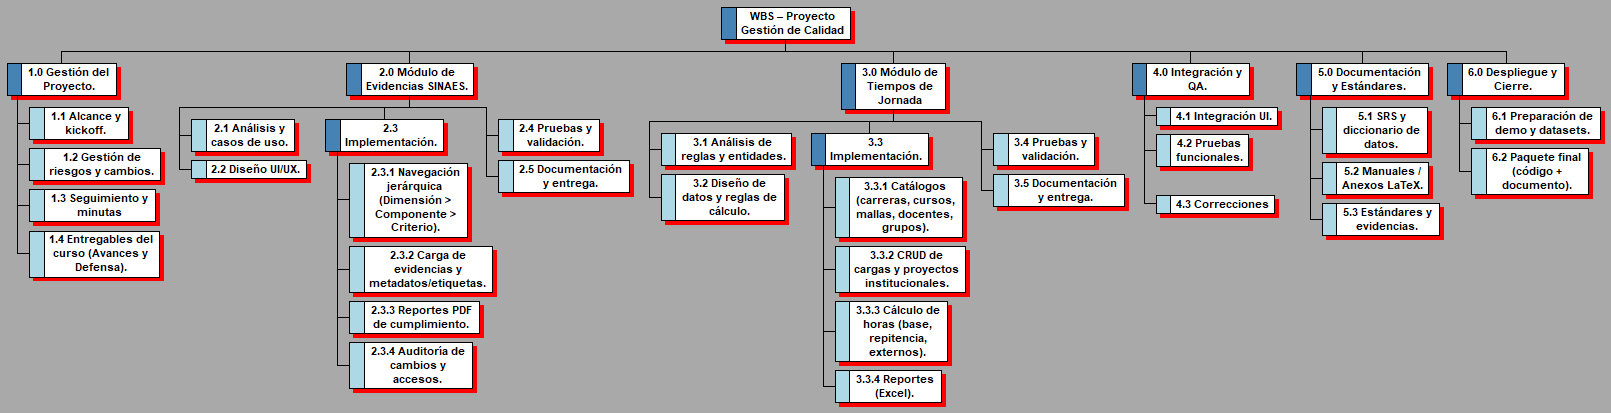
\includegraphics[width=\textwidth]{figs/wbs_chart.png}
  \caption{Estructura de Desglose del Trabajo (WBS) del proyecto.}
  \label{fig:wbs}
\end{figure}

Para referencia en alta resolución, el diagrama completo se incluye también en el \hyperref[anexo:wbs]{Anexo 7: WBS (Estructura de Desglose de Trabajo)}.

\subsection{Aplicación al proyecto}
La adaptación de Scrum al macro-proyecto \textbf{Gestión de Calidad} se realizó con los siguientes lineamientos:

\begin{itemize}
    \item \textbf{Roles:}
    \begin{itemize}
        \item \textbf{Product Owner (PO):} Comité de Calidad de la UNA y profesores responsables, quienes priorizan y validan entregables.
        \item \textbf{Scrum Master:} rol asumido de forma rotativa entre los estudiantes, garantizando disciplina metodológica.
        \item \textbf{Equipo de Desarrollo:} integrado por los 2 estudiantes responsables de la construcción de los módulos.
    \end{itemize}

    \item \textbf{Eventos:}
    \begin{itemize}
        \item \textbf{Sprint Planning:} definición de objetivos y tareas cada dos semanas.
        \item \textbf{Daily Scrum:} reuniones virtuales de 15 minutos para seguimiento y bloqueos.
        \item \textbf{Sprint Review:} demostración de los incrementos funcionales al PO al cierre de cada sprint.
        \item \textbf{Sprint Retrospective:} análisis del proceso y propuestas de mejora.
    \end{itemize}

    \item \textbf{Artefactos:}
    \begin{itemize}
        \item \textbf{Product Backlog:} listado priorizado de requerimientos funcionales (RF-01 al RF-17).
        \item \textbf{Sprint Backlog:} conjunto de tareas planificadas en cada sprint.
        \item \textbf{Incremento:} entregables funcionales validados al cierre de la iteración.
    \end{itemize}

    \item \textbf{Ajustes específicos:}
    \begin{itemize}
        \item \textbf{Duración de sprint:} 2 semanas, alineadas con los avances del curso.
        \item \textbf{Entregas formales:} vinculadas a los Avances 1, 2, 3 y a la Defensa Final.
        \item \textbf{Herramientas:} GitHub Projects para gestión de backlog, GitHub Actions para CI/CD y Google Drive para almacenamiento y evidencias.
    \end{itemize}
\end{itemize}

De esta forma, Scrum se implementa como una metodología realista y adaptable, con foco en entregas funcionales que aseguran el cumplimiento de los criterios académicos y de acreditación.
   % Metodología
\chapter{Estándares}

Con el fin de garantizar la calidad, mantenibilidad, seguridad y coherencia del macro-proyecto “Gestión de Calidad” (módulo de Evidencias SINAES y módulo de Tiempos de Jornada), se definen los siguientes estándares técnicos y metodológicos.

\section{Estándares de Documentación}
\begin{itemize}
    \item Uso de archivos \textbf{README.md} en cada repositorio con instrucciones claras de instalación, despliegue y contribución.
    \item Convención de \textbf{Conventional Commits} para los mensajes de confirmación en Git, asegurando trazabilidad de cambios.
    \item Documentación de APIs mediante \textbf{Swagger/OpenAPI 3.0}, facilitando la comprensión y consumo de los servicios.
    \item Manuales de usuario y anexos técnicos en formato \LaTeX, siguiendo la estructura institucional.
\end{itemize}

\section{Estándares de Programación}
\begin{itemize}
    \item \textbf{Frontend:} uso de TypeScript con ESLint (Airbnb Style Guide) y Prettier para asegurar consistencia en estilo de código.
    \item \textbf{Backend:} aplicación de arquitectura hexagonal y principios de Domain-Driven Design (DDD) en el módulo de Tiempos de Jornada.
    \item \textbf{Control de versiones:} adopción de \textbf{Git Flow} para la gestión de ramas (main, develop, feature, release, hotfix).
    \item \textbf{Pruebas unitarias:} Jest como framework estándar para validación automática de componentes y servicios.
\end{itemize}

\section{Estándares de Base de Datos}
\begin{itemize}
    \item \textbf{MongoDB} como base de datos NoSQL para el módulo de Tiempos de Jornada, seleccionada por su flexibilidad y escalabilidad.
    \item Uso de \textbf{Prisma ORM} como estándar de interacción entre backend y base de datos, asegurando tipado seguro y reducción de errores.
    \item \textbf{Google Drive API} como repositorio oficial de evidencias del módulo SINAES, con metadatos estandarizados para cada documento.
    \item Respaldos periódicos automatizados, siguiendo políticas institucionales de integridad y disponibilidad.
\end{itemize}

\section{Estándares de Interfaz}
\begin{itemize}
    \item \textbf{Shadcn UI} como librería de componentes estándar en el frontend, garantizando consistencia visual y accesibilidad.
    \item Cumplimiento de las pautas \textbf{WCAG 2.1 nivel AA}, asegurando accesibilidad para todos los usuarios.
    \item Diseño \textbf{responsive-first}, validado en dispositivos móviles, tabletas y escritorios.
    \item Uso de patrones de navegación jerárquica para facilitar el acceso a dimensiones, componentes y criterios en el módulo SINAES.
\end{itemize}
   % Estándares
\chapter{Costos y Factibilidad Económica}

\section{3.3.3. Factibilidad Económica}
Dado que se trata de un proyecto académico y sin fines de lucro, se opta por una estrategia de desarrollo de bajo costo. 
Se emplean herramientas y plataformas de uso libre o con planes académicos gratuitos, como GitHub para el control de versiones, MongoDB en su modalidad gratuita, y Google Drive para el almacenamiento de evidencias. 
El desarrollo se realiza de forma local en los equipos personales de los integrantes, distribuyendo las tareas según los módulos definidos en el WBS. 
Esta estrategia permite garantizar la continuidad del proyecto sin generar gastos adicionales a la institución.

\section{Costos de desarrollo}
El desarrollo se ejecuta dentro del marco del curso \textit{Ingeniería en Sistemas II} de la Universidad Nacional, 
por lo que no existen costos asociados a contratación o licencias de software. 
Todas las herramientas utilizadas son gratuitas y de libre acceso, y el despliegue de las pruebas se realiza en entornos locales. 
De requerirse demostraciones institucionales, estas se efectuarán mediante el uso de cuentas académicas o servidores internos de la UNA.

\section{Costos de capital humano}
Las actividades técnicas están a cargo del equipo de desarrollo estudiantil, compuesto por:

\begin{itemize}
  \item \textbf{Francisco Mora Cabezas:} Desarrollo del backend del módulo \textit{Tiempos de Jornada}, diseño y definición del esquema correspondiente, integración visual y elaboración de la documentación general del proyecto.
  \item \textbf{Ángel Segura Méndez:} Desarrollo del backend del módulo \textit{Evidencias SINAES}, modelado de su base de datos y elaboración de documentación técnica específica del módulo.
\end{itemize}

Cada integrante es responsable del ciclo completo de su módulo, incluyendo la lógica del backend, pruebas unitarias y coordinación para la integración futura entre ambos sistemas. 
No se contemplan remuneraciones, dado que el trabajo forma parte del proceso académico dentro del curso. 
La participación docente se limita a la supervisión, seguimiento metodológico y validación de los avances.


\section{Cargos administrativos}
El sistema está diseñado para operar completamente en línea o en entornos de prueba locales, eliminando la necesidad de documentación física. 
Por ello, los costos administrativos son prácticamente nulos. 
Se prevé únicamente el uso de materiales de apoyo o presentaciones digitales dentro del entorno académico.

\section{Costos totales del proyecto}
El proyecto puede desarrollarse sin generar costos monetarios directos. 
No obstante, se estima un gasto potencial máximo de ₡25\,000 a ₡30\,000 (aproximadamente 40–50 USD) en caso de requerir:
\begin{itemize}
  \item Compra de un dominio institucional para futuras pruebas públicas.
  \item Certificados SSL u otros servicios asociados al despliegue de pruebas.
\end{itemize}
Estos costos son opcionales y no forman parte de la presente etapa del proyecto.

\section{Resumen consolidado de costos}

A continuación se presenta una tabla consolidada que resume todos los costos asociados al desarrollo e implementación del Sistema de Gestión Integral Universitario:

\begin{table}[H]
\centering
\begin{tabular}{|l|r|p{5cm}|}
\hline
\textbf{Categoría de Costo} & \textbf{Monto (₡)} & \textbf{Observaciones} \\
\hline
\hline
\multicolumn{3}{|l|}{\textbf{I. Costos de Desarrollo}} \\
\hline
Herramientas y software & 0.00 & Uso de tecnologías open source \\
Plataformas (GitHub, MongoDB Free, Vercel) & 0.00 & Planes académicos gratuitos \\
IDE y entornos de desarrollo & 0.00 & VS Code, Node.js (gratuitos) \\
\hline
\textbf{Subtotal Desarrollo} & \textbf{0.00} & \\
\hline
\hline
\multicolumn{3}{|l|}{\textbf{II. Costos de Capital Humano}} \\
\hline
Desarrollo técnico (576 horas) & 0.00 & Proyecto académico \\
Supervisión docente & 0.00 & Dentro del curso ISII \\
Reuniones y coordinación & 0.00 & Herramientas virtuales gratuitas \\
\hline
\textbf{Subtotal Capital Humano} & \textbf{0.00} & \\
\hline
\hline
\multicolumn{3}{|l|}{\textbf{III. Costos Administrativos}} \\
\hline
Documentación física & 0.00 & Todo en formato digital \\
Comunicaciones & 0.00 & Google Meet, Discord, WhatsApp \\
Almacenamiento (Google Drive) & 0.00 & Cuentas académicas \\
\hline
\textbf{Subtotal Administrativo} & \textbf{0.00} & \\
\hline
\hline
\multicolumn{3}{|l|}{\textbf{IV. Costos Opcionales (Futuros)}} \\
\hline
Dominio institucional (.cr) & 10,000 - 15,000 & Si se requiere despliegue público \\
Certificado SSL & 5,000 - 10,000 & Si se requiere HTTPS personalizado \\
Hosting demo (opcional) & 0 - 10,000 & Alternativa: usar Vercel gratuito \\
\hline
\textbf{Subtotal Opcional} & \textbf{15,000 - 35,000} & \\
\hline
\hline
\textbf{TOTAL GARANTIZADO} & \textbf{₡0.00} & \textbf{Costo real del proyecto} \\
\textbf{TOTAL MÁXIMO ESTIMADO} & \textbf{₡35,000} & \textbf{Solo si se requieren servicios adicionales} \\
\hline
\end{tabular}
\caption{Consolidado General de Costos del Proyecto}
\label{tab:costos_consolidado}
\end{table}

\textbf{Nota importante sobre costo-beneficio:} 

Aunque el costo directo del proyecto es de ₡0.00, el valor generado es significativo. La Universidad Nacional actualmente invierte aproximadamente ₡58 millones anuales en gestión manual de evidencias SINAES (según estimaciones institucionales de horas-persona dedicadas a búsqueda, organización y auditoría de documentos). 

Adicionalmente, el módulo de Tiempos de Jornada optimiza un proceso que actualmente consume entre 40-60 horas por ciclo académico en cálculos manuales, revisiones y correcciones de asignaciones docentes. La automatización de este proceso representa un ahorro estimado de ₡2.4 millones anuales en productividad administrativa.

Por lo tanto, la relación costo-beneficio es extraordinariamente favorable: **inversión de ₡0.00 con retorno anual estimado de ₡60+ millones en ahorro de tiempo y optimización de recursos humanos**.

\section{Conclusiones de la factibilidad económica}
El proyecto es económicamente viable y presenta una relación costo-beneficio excepcional. 
Aprovecha herramientas gratuitas de código abierto, no requiere inversión inicial y mantiene un costo de mantenimiento prácticamente nulo. 
Al estar alineado con los principios de software libre y educación abierta, contribuye al fortalecimiento institucional sin demandar recursos financieros adicionales. 

El único costo potencial (₡15,000-₡35,000) surgiría únicamente si la institución decidiera en el futuro implementar un despliegue público con dominio personalizado, certificado SSL profesional y servicios premium de hosting. Sin embargo, este gasto sería completamente opcional, ya que el sistema puede operar indefinidamente con las herramientas gratuitas actuales.

En términos de costo-beneficio, la relación es altamente favorable: el impacto esperado —automatización, transparencia, eficiencia administrativa y ahorro de ₡60+ millones anuales— se logra con una inversión real de cero colones.
+++  % Costos
\chapter{Desarrollo}

\section{Introducción}
Este capítulo describe el proceso de desarrollo del \textbf{Sistema de Gestión Integral Universitario}, el cual contempla dos módulos principales: Gestión de Evidencias SINAES y Gestión de Tiempos de Jornada. El desarrollo se realiza de forma iterativa siguiendo la metodología Scrum, con entregas incrementales en cada sprint.

\section{Gestión de Reuniones y Documentación}

\subsection{Formato de Minutas de Reunión}
Durante el desarrollo del proyecto, se implementó un riguroso proceso de documentación de reuniones mediante minutas estructuradas, siguiendo el formato establecido en \hyperref[anexo:formato_minutas]{Anexo 6: Formato de minutas de reunión}. Estas minutas constituyeron una herramienta fundamental para:

\begin{itemize}
    \item Documentar decisiones técnicas y de negocio tomadas durante el desarrollo.
    \item Registrar acuerdos con los diferentes actores del proyecto.
    \item Establecer compromisos y fechas de entrega para cada sprint.
    \item Identificar problemas potenciales de manera temprana.
    \item Mantener la trazabilidad de los cambios solicitados.
\end{itemize}

Cada minuta siguió una estructura estandarizada que incluye:
\begin{enumerate}
    \item Información general (fecha, hora, lugar, participantes).
    \item Agenda de la reunión.
    \item Temas discutidos.
    \item Acuerdos alcanzados.
    \item Compromisos adquiridos.
    \item Próximos pasos.
    \item Firmas de los participantes.
\end{enumerate}

Este formato permitió mantener una comunicación efectiva entre el equipo de desarrollo y los usuarios finales del sistema (representantes de la UNA), asegurando que todas las partes interesadas estuvieran alineadas con los objetivos del proyecto.

\subsection{Gestión de Cambios}
Un aspecto crítico del desarrollo fue la implementación de un proceso formal de gestión de cambios, documentado a través de un formulario específico (ver \hyperref[anexo:formulario_gestion_de_cambios]{Anexo 12: Formulario gestión de cambios}). Este proceso permitió manejar de manera efectiva las modificaciones solicitadas durante el desarrollo, garantizando que:

\begin{itemize}
    \item Los cambios fueran evaluados en términos de impacto en alcance, tiempo y recursos.
    \item Se mantuviera la integridad del sistema a lo largo del desarrollo.
    \item Se priorizaran los cambios según su importancia y urgencia.
    \item Se documentaran adecuadamente las modificaciones realizadas.
    \item Se mantuviera la trazabilidad entre los requisitos originales y los cambios implementados.
\end{itemize}

\subsubsection{Actores Clave en la Gestión de Cambios}
Para asegurar un proceso de gestión de cambios efectivo y alineado con los objetivos del proyecto, se identificaron los siguientes actores clave cuya participación fue fundamental:

\begin{itemize}
    \item \textbf{Estudiantes (Equipo de Desarrollo):}
        \begin{itemize}
            \item Francisco Mora Cabezas
            \item Ángel Segura Méndez
        \end{itemize}
    \item \textbf{Profesor:} Saray Castro Mora
    \item \textbf{Cliente (Dueño del Producto):} Josías Chávez Murillo
\end{itemize}

Un principio fundamental establecido fue que para la aprobación de cualquier cambio se requería, como mínimo, el consenso entre los estudiantes y el profesor. Este requisito garantizó que todos los cambios fueran debidamente evaluados desde perspectivas académicas y técnicas antes de su implementación.

El proceso de gestión de cambios implementado constó de las siguientes etapas:

\begin{enumerate}
    \item \textbf{Solicitud de cambio:} Documentación formal de la modificación requerida, que podía ser iniciada por cualquiera de los actores clave.
    \item \textbf{Análisis de impacto:} Evaluación técnica y de recursos necesarios, realizada por los estudiantes con supervisión del profesor.
    \item \textbf{Aprobación:} Decisión basada en el análisis previo, requiriendo como mínimo el acuerdo entre estudiantes y profesor, e idealmente incluyendo al cliente.
    \item \textbf{Implementación:} Desarrollo e integración del cambio por parte del equipo de estudiantes.
    \item \textbf{Verificación:} Pruebas para asegurar que el cambio cumple los requisitos, con participación de todos los actores relevantes.
    \item \textbf{Documentación:} Actualización de la documentación del sistema y registro formal del cambio implementado.
\end{enumerate}

Esta metodología de gestión de cambios fue particularmente valiosa considerando la naturaleza iterativa del desarrollo, permitiendo incorporar mejoras y ajustes sin comprometer la calidad del producto final ni los plazos establecidos en el cronograma.

\section{Arquitectura Técnica}

El sistema se está desarrollando siguiendo una arquitectura moderna de tres capas, aplicando las mejores prácticas de la industria del software.

\subsection{Stack Tecnológico}

La selección del stack tecnológico se realizó en base a criterios de escalabilidad, mantenibilidad, compatibilidad con tecnologías actuales y disponibilidad de documentación:

\begin{itemize}
    \item \textbf{Frontend:} Next.js 15.1.0 con React 19.0.0, utilizando el patrón App Router para enrutamiento del lado del servidor.
    \item \textbf{Backend:} NestJS 10.4.19, framework de Node.js que implementa arquitectura hexagonal y principios SOLID.
    \item \textbf{Base de Datos:} MongoDB con Prisma ORM 6.10.1, aprovechando la flexibilidad de bases de datos NoSQL para esquemas evolutivos.
    \item \textbf{Autenticación:} JWT (JSON Web Tokens) con Passport.js, incluyendo integración con Google OAuth2.
    \item \textbf{UI/UX:} shadcn/ui + Tailwind CSS 3.4.16 para interfaces responsivas y accesibles.
    \item \textbf{Gestión de Estado:} Zustand 4.5.4 para state management del lado del cliente.
    \item \textbf{Validación:} Zod 3.24.2 + class-validator para validación de datos tanto en frontend como backend.
    \item \textbf{Documentación API:} Swagger/OpenAPI automático integrado en NestJS.
\end{itemize}

\subsection{Arquitectura Monorepo}

El proyecto se organiza como un monorepo gestionado por pnpm workspaces y Turbo, lo que permite:

\begin{itemize}
    \item Compartir código común entre frontend y backend (tipos TypeScript, validaciones).
    \item Gestionar dependencias de manera centralizada.
    \item Ejecutar builds incrementales y paralelos.
    \item Mantener consistencia en estándares de código mediante ESLint compartido.
\end{itemize}

\textbf{Estructura del monorepo:}

\begin{quote}
\texttt{Gestion\_Calidad/}\\
\hspace*{1em}\texttt{apps/}\\
\hspace*{2em}\texttt{backend/} \hspace{2em}\textit{\# API NestJS}\\
\hspace*{2em}\texttt{frontend/} \hspace{1.5em}\textit{\# App Next.js}\\
\hspace*{2em}\texttt{docs/} \hspace{2.8em}\textit{\# Documentación Docusaurus}\\
\hspace*{1em}\texttt{packages/}\\
\hspace*{2em}\texttt{database/} \hspace{1.5em}\textit{\# Prisma schemas compartidos}\\
\hspace*{2em}\texttt{ui/} \hspace{3.3em}\textit{\# Componentes React reutilizables}\\
\hspace*{2em}\texttt{eslint-config/} \hspace{0.3em}\textit{\# Configuraciones de linting}\\
\hspace*{2em}\texttt{typescript-config/} \textit{\# tsconfig base}
\end{quote}

\section{Módulo de Evidencias SINAES}

\subsection{Descripción y Cliente}

El módulo de Gestión de Evidencias SINAES tiene como cliente principal al Lic. Josías Chávez Murillo. Este módulo busca centralizar y organizar toda la documentación probatoria requerida por el Sistema Nacional de Acreditación de la Educación Superior (SINAES).

\subsection{Componentes Principales}

El módulo contempla las siguientes entidades y funcionalidades:

\begin{itemize}
    \item \textbf{Gestión de Dimensiones SINAES:} Administración de las dimensiones y componentes definidos por SINAES.
    \item \textbf{Tipos de Documentos:} Categorización de documentos según estándares institucionales.
    \item \textbf{Carga de Evidencias:} Subida y almacenamiento de documentos probatorios en Google Drive.
    \item \textbf{Consulta de Evidencias:} Búsqueda avanzada de documentos por dimensión, componente, criterio y año.
    \item \textbf{Definición de Criterios:} Establecimiento de criterios de cumplimiento para cada componente SINAES.
    \item \textbf{Auditoría:} Registro de cambios y modificaciones a documentos.
\end{itemize}

\subsection{Estructura de Backend}

El backend del módulo SINAES incluye los siguientes módulos NestJS:

\begin{itemize}
    \item \texttt{DimensionsModule}: CRUD de dimensiones SINAES.
    \item \texttt{ComponentsModule}: Gestión de componentes por dimensión.
    \item \texttt{CriteriaModule}: Definición y administración de criterios de evaluación.
    \item \texttt{EvidencesModule}: Carga, almacenamiento y consulta de evidencias documentales.
    \item \texttt{DocumentTypesModule}: Categorización de tipos de documentos.
    \item \texttt{GoogleDriveModule}: Integración con API de Google Drive para almacenamiento.
\end{itemize}

\subsection{Interfaz de Usuario}

La interfaz del módulo SINAES proporciona vistas para:

\begin{itemize}
    \item Dashboard con resumen de evidencias por dimensión.
    \item Formulario de carga de documentos con validación.
    \item Buscador avanzado con filtros múltiples.
    \item Vista de árbol jerárquico (Dimensión > Componente > Criterio > Evidencias).
    \item Gestión de permisos por rol (administrador, coordinador, docente).
\end{itemize}

\section{Módulo de Tiempos de Jornada}

\subsection{Descripción y Cliente}

El módulo de Gestión de Tiempos de Jornada tiene como cliente principal al Lic. Erick Madrigal. Este módulo automatiza el cálculo y distribución de las cargas académicas docentes según los tiempos de jornada establecidos por la institución.

\subsection{Componentes Principales}

El módulo contempla las siguientes funcionalidades:

\begin{itemize}
    \item \textbf{Configuración de Rangos:} Definición de rangos de horas para cada tipo de jornada (1/4, 1/2, 3/4, tiempo completo).
    \item \textbf{Presupuesto Anual:} Asignación del presupuesto total de tiempos de jornada por año académico.
    \item \textbf{Distribución por Campus:} Asignación de tiempos de jornada a diferentes sedes universitarias.
    \item \textbf{Asignaciones Docentes:} Registro de cargas académicas individuales (cursos, proyectos, tareas administrativas).
    \item \textbf{Proyectos Institucionales:} Gestión de proyectos que requieren tiempo de jornada docente.
    \item \textbf{Proveedores Externos:} Administración de convenios que aportan tiempos adicionales.
\end{itemize}

\subsection{Modelo de Datos}

El modelo de datos incluye seis entidades principales en MongoDB:

\begin{enumerate}
    \item \textbf{JourneyTimeCalculationConfig:} Almacena los rangos de horas y valores para cada tipo de jornada (1/4, 1/2, 3/4, Tiempo Completo).
    \item \textbf{AnnualJourneyTimeAllocation:} Gestiona el presupuesto anual de tiempos de jornada por sede.
    \item \textbf{CampusJourneyTimeAllocation:} Distribuye los tiempos entre sedes específicas, calculando automáticamente tiempos disponibles.
    \item \textbf{ProfessorAssignment:} Registra asignaciones individuales de profesores a cursos, proyectos o tareas administrativas.
    \item \textbf{InstitutionalProject:} Modela proyectos institucionales que consumen tiempos de jornada.
    \item \textbf{ExternalProvider:} Gestiona proveedores externos (convenios) que aportan tiempos adicionales.
\end{enumerate}

El modelo completo se encuentra documentado en el \hyperref[anexo:dicc_jornada]{Anexo 15: Diccionario de Datos --- Tiempos de Jornada} y \hyperref[anexo:modelo_no_relacional]{Anexo 9: Modelo No Relacional}.

\subsection{Estructura de Backend}

El backend del módulo de Tiempos de Jornada contempla los siguientes módulos NestJS:

\begin{itemize}
    \item \texttt{JourneyTimeConfigsModule}: Gestión de configuraciones de rangos de horas para cada tipo de jornada.
    \item \texttt{AnnualJourneyTimeAllocationsModule}: Administración del presupuesto anual de tiempos de jornada.
    \item \texttt{CampusJourneyTimeAllocationsModule}: Distribución de tiempos entre campus con cálculo automático de disponibilidad.
    \item \texttt{ProfessorAssignmentsModule}: Registro de asignaciones docentes individuales.
    \item \texttt{ExternalProvidersModule}: Gestión de proveedores externos y convenios.
    \item \texttt{InstitutionalProjectsModule}: Administración de proyectos institucionales.
\end{itemize}

\subsubsection{Lógica de Cálculo}

El sistema implementa cálculo automático de tiempos de jornada según las horas trabajadas. La disponibilidad de tiempos en cada campus se calcula mediante la fórmula:

\begin{center}
\texttt{disponible = asignado + adicional - consumido}
\end{center}

Esto permite mantener control automático de la disponibilidad de recursos en cada campus.

\subsection{Interfaz de Usuario}

La interfaz del módulo de Tiempos de Jornada incluye:

\begin{itemize}
    \item Dashboard con resumen de distribución de tiempos por campus.
    \item Configuración de rangos de jornada (1/4, 1/2, 3/4, tiempo completo).
    \item Calculadora interactiva de tipos de jornada según horas trabajadas.
    \item Gestión de asignaciones docentes individuales.
    \item Registro de proyectos institucionales y proveedores externos.
    \item Reportes de consumo y disponibilidad por campus y ciclo académico.
\end{itemize}

\section{Integración entre Módulos}

Ambos módulos comparten infraestructura común:

\begin{itemize}
    \item \textbf{Autenticación:} Sistema unificado con JWT y Google OAuth2.
    \item \textbf{Base de Datos:} MongoDB compartida con esquemas separados por módulo.
    \item \textbf{Gestión de Roles:} Permisos diferenciados (administrador, coordinador, docente).
    \item \textbf{Auditoría:} Registro centralizado de cambios para ambos módulos.
    \item \textbf{API Gateway:} Punto único de entrada para servicios backend.
\end{itemize}

\section{Estado Actual del Desarrollo}

El desarrollo se encuentra en progreso continuo, con entregas incrementales en cada sprint. Las funcionalidades base de ambos módulos están implementadas, y se continúa trabajando en:

\begin{itemize}
    \item Validaciones avanzadas en formularios.
    \item Mejoras en búsquedas y filtros.
    \item Reportes de cumplimiento y auditoría.
    \item Optimización de rendimiento.
    \item Documentación técnica y de usuario.
\end{itemize}

\section{Implementación y Despliegue}

\subsection{Plan de Implementación del Sistema}

La implementación del \textbf{Sistema de Gestión Integral Universitario} se planificó en función de los sprints definidos en el cronograma del proyecto, siguiendo un enfoque incremental que permitió integrar los módulos de Evidencias SINAES y Tiempos de Jornada de manera progresiva sobre una infraestructura común. El plan contempla las siguientes etapas:

\begin{enumerate}
    \item \textbf{Preparación del entorno:} Configuración del monorepo (pnpm + Turbo), provisión de bases de datos MongoDB, generación de credenciales OAuth2 de Google Drive y configuración de variables de entorno por ambiente.
    \item \textbf{Construcción incremental:} Desarrollo y entrega por sprints, integrando primero la base de autenticación y seguridad, luego el módulo de Evidencias SINAES y finalmente el módulo de Tiempos de Jornada.
    \item \textbf{Integración continua:} Cada cambio se valida con linters (ESLint), formateo (Prettier), verificación de tipos (TypeScript) y pruebas automatizadas (Jest) antes de fusionarse a la rama principal.
    \item \textbf{Despliegue a ambientes:} Promoción controlada desde el ambiente de desarrollo local hacia el ambiente de pruebas (QA) y, posteriormente, al ambiente de producción alojado en el servidor Hetzner.
    \item \textbf{Verificación post-despliegue:} Revisión de bitácoras de los contenedores, pruebas de humo sobre los endpoints críticos y validación funcional de los flujos principales.
\end{enumerate}

\subsection{Estrategia de Despliegue y Ambientes Definidos}

El sistema se despliega bajo una arquitectura contenedorizada con Docker y orquestada mediante \texttt{docker-compose}. Se utiliza Traefik 2.11 como proxy reverso, con resolución automática de certificados TLS mediante Let's Encrypt (HTTP-01 challenge) y cabeceras de seguridad gestionadas por archivos dinámicos de configuración.

\subsubsection{Ambiente de Desarrollo}
\begin{itemize}
    \item \textbf{Ubicación:} Estaciones de trabajo locales del equipo de desarrollo.
    \item \textbf{Ejecución:} \texttt{pnpm run dev} levanta backend (NestJS) y frontend (Next.js) en modo hot-reload, junto con el servidor de documentación Docusaurus.
    \item \textbf{Base de datos:} Instancia MongoDB local (o cluster de desarrollo) gestionada con Prisma.
    \item \textbf{Propósito:} Implementación y prueba de funcionalidades, depuración y validación temprana del comportamiento.
\end{itemize}

\subsubsection{Ambiente de Pruebas (QA)}
\begin{itemize}
    \item \textbf{Ubicación:} Construcción Docker equivalente a producción, ejecutada en una rama o instancia separada.
    \item \textbf{Datos:} Conjunto controlado de datos de prueba que replica escenarios reales sin comprometer información sensible.
    \item \textbf{Propósito:} Validación funcional, pruebas de integración, pruebas de regresión y revisión por parte del cliente antes de cada liberación.
\end{itemize}

\subsubsection{Ambiente de Producción}
\begin{itemize}
    \item \textbf{Infraestructura:} Servidor dedicado en Hetzner, red Docker aislada \texttt{gcalidad-network} (\texttt{172.30.0.0/24}).
    \item \textbf{Servicios:} Contenedores \texttt{agr-frontend} (Next.js), \texttt{agr-backend} (NestJS) y \texttt{traefik} actuando como proxy y terminador TLS.
    \item \textbf{Dominios:} Frontend expuesto en \texttt{gestion-calidad.arayaroma.software} y API en \texttt{api-gestion-calidad.arayaroma.software}, con redirección automática HTTP $\rightarrow$ HTTPS.
    \item \textbf{Almacenamiento de archivos:} Google Drive como repositorio documental para las evidencias SINAES, mediante una cuenta de servicio con acceso restringido.
\end{itemize}

\subsection{Procedimiento de Instalación y Configuración}

El despliegue automatizado se realiza mediante el script \texttt{deploy-hetzner.sh}, que sincroniza el código fuente con el servidor remoto y reconstruye los contenedores. El procedimiento general es el siguiente:

\begin{enumerate}
    \item \textbf{Requisitos previos:} Node.js $\geq$ 18.x, pnpm $\geq$ 8.x, Docker y Docker Compose instalados en el servidor.
    \item \textbf{Clonado y configuración:} Obtención del repositorio y creación de los archivos \texttt{.env}, \texttt{apps/backend/.env.production} y \texttt{apps/frontend/.env.production} con las credenciales correspondientes (cadena de conexión a MongoDB, secretos JWT, credenciales Google OAuth2, dominios públicos).
    \item \textbf{Sincronización:} \texttt{./deploy-hetzner.sh all} ejecuta \texttt{rsync} excluyendo \texttt{node\_modules}, \texttt{.next}, \texttt{dist}, \texttt{.git} y archivos sensibles locales.
    \item \textbf{Construcción de imágenes:} \texttt{docker compose build --no-cache} reconstruye las imágenes de \texttt{frontend} y \texttt{backend}.
    \item \textbf{Levantamiento de servicios:} \texttt{docker compose up -d} inicia los contenedores con sus etiquetas Traefik para enrutamiento y certificados.
    \item \textbf{Verificación:} Inspección de \texttt{docker compose ps} y de las bitácoras (\texttt{docker logs agr-frontend}, \texttt{docker logs agr-backend}) para confirmar el inicio correcto.
    \item \textbf{Migración de esquemas:} Ejecución de \texttt{pnpm run prisma} para generar y aplicar los esquemas de Prisma sobre la base de datos.
\end{enumerate}

\subsection{Plan de Respaldos y Recuperación}

Dado que el sistema gestiona información crítica para la acreditación SINAES y la planificación académica, se define una estrategia de respaldos en dos planos:

\begin{itemize}
    \item \textbf{Base de datos (MongoDB):} Respaldos automatizados mediante \texttt{mongodump} con periodicidad diaria (incrementales) y semanal (completos), almacenados de forma cifrada y conservados por al menos 30 días. Las restauraciones se prueban periódicamente sobre un ambiente aislado para validar la integridad de los volcados.
    \item \textbf{Documentos probatorios (Google Drive):} La propia plataforma de Google Drive provee versionado y papelera con periodo de retención. Adicionalmente, se documenta una jerarquía de carpetas controlada por el módulo \texttt{GoogleDriveFolders}, lo que permite reconstruir la estructura ante eliminaciones accidentales.
    \item \textbf{Configuración e infraestructura:} El \texttt{docker-compose.yml}, los archivos de Traefik (\texttt{headers.yml}, \texttt{redirect.yml}, \texttt{tls.yml}) y los certificados de Let's Encrypt (volumen \texttt{traefik\_certs}) se versionan o respaldan para permitir la reconstrucción rápida del entorno.
    \item \textbf{Procedimiento de recuperación:} En caso de incidente se restaura primero la infraestructura base (servidor, red Docker, Traefik), luego la base de datos a partir del último respaldo válido y, finalmente, se redespliega la aplicación mediante \texttt{deploy-hetzner.sh}.
\end{itemize}

\subsection{Capacitación al Usuario Final y Entrega de Manuales}

La estrategia de capacitación se concibió en dos frentes, alineados con los perfiles de usuario del sistema:

\begin{itemize}
    \item \textbf{Capacitación funcional:} Sesiones dirigidas a los usuarios clave (Lic. Josías Chávez Murillo para el módulo SINAES y Lic. Erick Madrigal para el módulo de Tiempos de Jornada), cubriendo los flujos de carga de evidencias, configuración de rangos de jornada, registro de asignaciones docentes y consulta de reportes.
    \item \textbf{Material entregable:} Documentación funcional y técnica generada con Docusaurus (\texttt{apps/docs}), accesible vía \texttt{pnpm --filter @una-gc/docs start} en \texttt{http://localhost:5000}, complementada con la documentación API auto-generada por Swagger/OpenAPI desde el backend NestJS.
    \item \textbf{Manuales:} Manual de usuario por módulo, manual de administrador (gestión de roles y permisos) y manual técnico de despliegue, todos versionados dentro del propio monorepo.
\end{itemize}

\section{Aceptación por Parte del Usuario}

\subsection{Plan de Pruebas de Aceptación del Usuario (UAT)}

El plan de UAT se diseñó para validar, en condiciones reales de uso, que el sistema cumple con los requerimientos definidos en el SRS (\hyperref[anexo:documento_srs]{Anexo 8}). Contempla:

\begin{itemize}
    \item \textbf{Alcance:} Validación de los flujos críticos de ambos módulos: autenticación con Google OAuth2, carga y búsqueda de evidencias SINAES, configuración de rangos de jornada, registro de asignaciones docentes y generación de reportes.
    \item \textbf{Criterios de aceptación:} Cumplimiento de los requerimientos funcionales del SRS, ausencia de defectos bloqueantes, tiempos de respuesta razonables en operaciones cotidianas y consistencia entre la información mostrada en la interfaz y la almacenada en MongoDB / Google Drive.
    \item \textbf{Roles participantes:} Cliente / Dueño del Producto (Lic. Josías Chávez Murillo y Lic. Erick Madrigal), Profesor responsable (Saray Castro Mora) y Equipo de Desarrollo.
    \item \textbf{Casos de prueba:} Conjunto derivado de las historias de usuario, ejecutados sobre el ambiente de QA con datos de prueba representativos.
\end{itemize}

\subsection{Ejecución y Evidencias de las Pruebas}

La ejecución de las pruebas de aceptación se realizó en sesiones conjuntas con los clientes sobre el ambiente desplegado. Las evidencias técnicas se recopilan en el \hyperref[anexo:desarrollo]{Anexo 13: Desarrollo}, que contiene capturas de las vistas funcionales del sistema. Adicionalmente, el repositorio cuenta con una suite de pruebas automatizadas (Jest) que respalda la validación funcional ejecutada por el usuario, con reportes de cobertura disponibles vía \texttt{pnpm --filter @una-gc/backend test:cov}.

\subsection{Bitácora de Hallazgos y Correcciones Aplicadas}

Durante el desarrollo se mantuvo un proceso continuo de auditoría técnica del módulo SINAES, formalizado en el documento \texttt{SINAES\_AUDIT.md} dentro del repositorio. Esta bitácora documenta:

\begin{itemize}
    \item Inconsistencias críticas (duplicaciones de componentes, código stub en producción).
    \item Errores de manejo de errores y casos borde (validaciones faltantes, \texttt{catch} silenciosos).
    \item Recomendaciones de remediación con su correspondiente prioridad.
\end{itemize}

Las correcciones se gestionaron a través del proceso formal de gestión de cambios descrito al inicio del capítulo, dejando registro en commits del repositorio y en el plan de remediación \texttt{SINAES\_FIX\_PLAN.md}.

\subsection{Acta de Aceptación}

El acta o carta formal de aceptación firmada por el usuario se incorpora como anexo del documento una vez completada la ejecución de la UAT en presencia del cliente y del profesor responsable (ver \hyperref[anexo:carpeta_firmas]{Anexo 12: Carpeta de firmas}).

\section{Desafíos}

\subsection{Desafíos Técnicos Enfrentados}

Durante el desarrollo se enfrentaron varios desafíos relevantes:

\begin{itemize}
    \item \textbf{Integración con Google Drive:} Manejo de cuotas de la API, autenticación OAuth2 con cuenta de servicio, sincronización entre la jerarquía documental en Drive y la base de datos, y construcción de un mecanismo de verificación de consistencia (\texttt{DriveSyncCheckerService}).
    \item \textbf{Modelado de la jerarquía SINAES:} Representación en MongoDB de una estructura de 5 niveles (Dimensiones $\rightarrow$ Componentes $\rightarrow$ Criterios $\rightarrow$ Estándares/Evidencias Directas $\rightarrow$ Evidencias de Calidad) preservando integridad referencial sobre un motor NoSQL.
    \item \textbf{Cálculo de tiempos de jornada:} Implementación de la fórmula \texttt{disponible = asignado + adicional - consumido} con consistencia transaccional sobre múltiples entidades (configuración, presupuesto anual, distribución por campus, asignaciones docentes).
    \item \textbf{Monorepo multi-app:} Coordinación de dependencias compartidas, builds incrementales y configuración unificada de ESLint/TypeScript entre backend, frontend, paquetes UI y documentación.
    \item \textbf{Despliegue contenedorizado:} Configuración de Traefik con resolución automática de certificados TLS, cabeceras de seguridad y enrutamiento dual HTTP/HTTPS para frontend y backend bajo dominios distintos.
\end{itemize}

\subsection{Riesgos Materializados y Acciones de Mitigación}

\begin{itemize}
    \item \textbf{Inconsistencias en código de producción:} Se detectaron componentes de depuración (\texttt{scroll-debug}, \texttt{config-debug}) y duplicaciones de archivos críticos en el módulo SINAES. \textbf{Mitigación:} formalización de la auditoría en \texttt{SINAES\_AUDIT.md}, definición del plan de remediación en \texttt{SINAES\_FIX\_PLAN.md} y aislamiento de utilidades de depuración detrás de \texttt{NODE\_ENV === 'development'}.
    \item \textbf{Funcionalidad parcial en sincronización con Drive:} El servicio \texttt{DriveSyncCheckerService} operaba como \emph{stub} y retornaba un estado optimista. \textbf{Mitigación:} priorización de la implementación real y bloqueo de la operación en producción mientras se cierra el hallazgo.
    \item \textbf{Dependencia de servicios externos (Google Drive, Let's Encrypt):} Disponibilidad sujeta a terceros. \textbf{Mitigación:} manejo de reintentos con backoff exponencial, monitoreo de cuotas y persistencia de los certificados en un volumen Docker (\texttt{traefik\_certs}).
\end{itemize}

\subsection{Cambios de Alcance y su Impacto}

Los cambios solicitados durante el desarrollo se canalizaron a través del Formulario de Gestión de Cambios (\hyperref[anexo:formulario_gestion_de_cambios]{Anexo 11}), evaluando en cada caso el impacto en alcance, cronograma y recursos. La metodología iterativa (Scrum) permitió absorber estos cambios en sprints siguientes sin comprometer la fecha de entrega general del proyecto.

\subsection{Lecciones Aprendidas}

\begin{itemize}
    \item Mantener una \textbf{auditoría técnica continua} (no solo al cierre) detecta inconsistencias antes de que se conviertan en deuda crítica.
    \item Las \textbf{verificaciones automatizadas} (linters, type-check, pruebas unitarias, cobertura) son indispensables en un monorepo donde un cambio puede impactar varias aplicaciones.
    \item Documentar la \textbf{infraestructura como código} (\texttt{docker-compose}, scripts de despliegue) acelera la recuperación ante incidentes y la incorporación de nuevos integrantes al equipo.
    \item La \textbf{comunicación frecuente con los clientes} (Lic. Chávez y Lic. Madrigal) permitió ajustar prioridades de forma temprana y evitar reprocesos.
    \item Disociar lógica de almacenamiento (Google Drive) de lógica de negocio (MongoDB/Prisma) facilitó las pruebas y la evolución independiente de cada componente.
\end{itemize}

\section{Detalles Técnicos}

\subsection{Arquitectura del Sistema}

El sistema sigue una arquitectura de tres capas desplegada como microservicios contenedorizados detrás de un proxy reverso:

\begin{itemize}
    \item \textbf{Capa de presentación:} Aplicación Next.js (App Router) que consume la API REST mediante un cliente HTTP centralizado, con estado global gestionado por Zustand y caché de servidor con React Query.
    \item \textbf{Capa de aplicación:} API NestJS modular, con módulos independientes por dominio (más de 50 módulos en \texttt{apps/backend/src/modules/}, agrupados por las áreas SINAES, Tiempos de Jornada, autenticación, parametrización y soporte).
    \item \textbf{Capa de datos:} MongoDB accedido vía Prisma ORM con esquemas compartidos en el paquete \texttt{@una-gc/database}, complementado por Google Drive como almacén de objetos documentales.
\end{itemize}

El diagrama detallado de componentes está disponible en el \hyperref[anexo:diseno]{Anexo 18: Diseño}, junto con los diagramas específicos de cada módulo (\hyperref[anexo:anexo19]{Anexo 19} y \hyperref[anexo:anexo20]{Anexo 20}).

\subsection{Tecnologías, Lenguajes y Frameworks Utilizados}

\begin{itemize}
    \item \textbf{Lenguajes:} TypeScript (frontend, backend y paquetes compartidos), JavaScript (scripts de soporte), SQL/MongoDB Query Language para consultas.
    \item \textbf{Frontend:} Next.js 15.1.0, React 19.0.0, Tailwind CSS 3.4.16, shadcn/ui, Zustand 4.5.4, React Query.
    \item \textbf{Backend:} NestJS 10.4.19, Prisma ORM 6.10.1, Passport.js, JWT, Zod 3.24.2, class-validator.
    \item \textbf{Persistencia:} MongoDB.
    \item \textbf{Integraciones externas:} Google Drive API (\texttt{googleapis}), Google OAuth2.
    \item \textbf{Tooling:} pnpm workspaces, Turbo, ESLint, Prettier, Husky (hooks de git), Jest (pruebas unitarias y de integración), Docusaurus (documentación).
    \item \textbf{Infraestructura:} Docker, Docker Compose, Traefik 2.11, Let's Encrypt, servidor Hetzner.
\end{itemize}

\subsection{Repositorio del Código Fuente y Control de Versiones}

El código fuente se gestiona en un repositorio Git con flujo de trabajo basado en ramas por funcionalidad y revisiones por pares antes de fusión a la rama principal. Aspectos relevantes del control de versiones:

\begin{itemize}
    \item \textbf{Estructura:} monorepo con apps (\texttt{backend}, \texttt{frontend}, \texttt{docs}) y paquetes (\texttt{database}, \texttt{ui}, \texttt{eslint-config}, \texttt{typescript-config}).
    \item \textbf{Hooks pre-commit:} configurados con Husky para ejecutar linters, formateadores y verificaciones de ortografía técnica (\texttt{cspell.config.yaml}).
    \item \textbf{Convenciones de commits:} mensajes descriptivos en español/inglés vinculados a tareas e issues del cronograma de sprints.
    \item \textbf{Equipo y contribuyentes:} Juan C. Camacho Solano, Fran Mora Cabezas, Ángel Stward Segura Méndez y Esteban Javier Granados Sibaja.
\end{itemize}

\subsection{Estándares de Codificación Aplicados}

\begin{itemize}
    \item \textbf{Linting:} configuración compartida en \texttt{@una-gc/eslint-config} para asegurar consistencia entre paquetes.
    \item \textbf{Tipado estricto:} TypeScript con \texttt{strict} habilitado, tipos compartidos publicados en paquetes internos.
    \item \textbf{Arquitectura:} principios SOLID en NestJS, separación módulo/servicio/controlador, repositorios para acceso a datos.
    \item \textbf{Validación:} DTOs validados con \texttt{class-validator} en backend y esquemas Zod en frontend.
    \item \textbf{Pruebas:} Jest con generación incremental de pruebas por fases (\texttt{generate\_tests\_phase*.sh}) y reportes de cobertura.
    \item \textbf{Estilo:} Prettier para formateo automático y reglas de nomenclatura consistentes (kebab-case en archivos, camelCase en variables, PascalCase en componentes y clases).
\end{itemize}

\subsection{Requerimientos de Hardware y Software para la Ejecución}

\textbf{Servidor de producción (mínimo recomendado):}
\begin{itemize}
    \item CPU: 2 vCPU.
    \item Memoria RAM: 4 GB.
    \item Almacenamiento: 40 GB SSD para sistema, imágenes Docker y volúmenes persistentes.
    \item Sistema operativo: Linux con Docker Engine y Docker Compose v2.
    \item Conectividad: IP pública con puertos 80 y 443 abiertos, registros DNS apuntando a los dominios del frontend y del backend.
\end{itemize}

\textbf{Estación de desarrollo:}
\begin{itemize}
    \item Node.js $\geq$ 18.x y pnpm $\geq$ 8.x.
    \item Docker Desktop o equivalente para pruebas locales contenedorizadas.
    \item Acceso a MongoDB local o a un cluster de desarrollo.
\end{itemize}

\textbf{Cliente final:} navegador moderno (Chrome, Firefox, Edge o Safari en sus versiones recientes) con JavaScript habilitado.

\subsection{Seguridad: Autenticación, Autorización y Manejo de Datos Sensibles}

\subsubsection{Autenticación}
\begin{itemize}
    \item Inicio de sesión mediante JWT firmado, gestionado con Passport.js dentro del módulo \texttt{auth} del backend.
    \item Integración con Google OAuth2 para el flujo de autenticación federada, requerido también para autorizar el acceso a Google Drive en nombre del usuario.
    \item Tokens almacenados de forma segura en el cliente y renovados según política definida en el backend.
\end{itemize}

\subsubsection{Autorización}
\begin{itemize}
    \item Modelo de roles diferenciados (administrador, coordinador, docente) implementado en los módulos \texttt{user-roles} y \texttt{user-permissions}.
    \item \emph{Guards} y decoradores específicos de NestJS protegen los endpoints sensibles (\texttt{apps/backend/src/modules/auth/guards} y \texttt{decorators}).
    \item Permisos verificados tanto en el backend (autoridad final) como en el frontend (para condicionar la interfaz).
\end{itemize}

\subsubsection{Manejo de Datos Sensibles}
\begin{itemize}
    \item \textbf{Cifrado en tránsito:} TLS terminado en Traefik con certificados Let's Encrypt y redirección forzada de HTTP a HTTPS.
    \item \textbf{Cabeceras de seguridad:} configuradas en \texttt{traefik/headers.yml} (HSTS, anti-clickjacking, protección contra MIME-sniffing).
    \item \textbf{Secretos:} variables de entorno gestionadas por archivos \texttt{.env} fuera del repositorio, con plantillas controladas.
    \item \textbf{Credenciales de servicio:} cuenta de servicio Google con permisos mínimos sobre Drive, almacenada como archivo JSON fuera del bundle de la imagen.
    \item \textbf{Auditoría:} registro centralizado de cambios en módulos clave (\texttt{sinaes-document-history}, \texttt{observations}, \texttt{project-logs}) para trazabilidad de acciones sensibles.
    \item \textbf{Aislamiento de red:} contenedores en una red Docker dedicada (\texttt{gcalidad-network}) sin exposición directa, expuestos únicamente a través del proxy.
\end{itemize}

   % Desarrollo
\chapter{Conclusiones}

El proyecto del **Sistema de Gestión Integral Universitario**, actualmente en sus fases iniciales de planificación y definición de requerimientos, se perfila como una solución estratégica para la Universidad Nacional. Tras la etapa de análisis preliminar y la consolidación de la Especificación de Requerimientos de Software (SRS), se pueden establecer las siguientes conclusiones sobre su potencial y el camino a seguir:

\begin{itemize}
    \item \textbf{Viabilidad y Pertinencia del Proyecto:} Se ha confirmado la viabilidad técnica y operativa del Sistema de Gestión Integral Universitario, el cual responde a necesidades críticas identificadas en la gestión de evidencias para acreditación SINAES y la administración de tiempos de jornada universitaria. Este proyecto es pertinente y fundamental para la modernización y optimización de procesos académicos y administrativos clave de la UNA.

    \item \textbf{Claridad en la Definición de Requerimientos:} A través de un proceso riguroso de recopilación y consolidación, se ha logrado definir una Especificación de Requerimientos de Software (SRS) completa, coherente y suficientemente detallada para guiar las próximas fases de diseño y desarrollo. Los requerimientos funcionales y no funcionales de ambos módulos han sido claros y validados con los usuarios clave.

    \item \textbf{Alineación con Estándares y Metodologías Modernas:} La adopción de metodologías ágiles como Scrum y el uso de estándares de desarrollo y seguridad modernos (React/Next.js, NestJS, MongoDB, Prisma, Google Drive API, JWT, AES-256) proveen una base tecnológica y de gestión robusta para el proyecto, prometiendo un desarrollo eficiente y de alta calidad.

    \item \textbf{Potencial de Impacto Significativo:} Se proyecta que el sistema contribuirá a la reducción de tiempos administrativos (ej. clasificación de evidencias), la eliminación de duplicidades, la mejora en la precisión de la planificación de recursos humanos y el fortalecimiento de la trazabilidad y seguridad de la información institucional. Estos beneficios son cruciales para los procesos de acreditación y la eficiencia operativa de la UNA.

    \item \textbf{Base para Futuras Fases:} Los requerimientos definidos y la arquitectura modular propuesta para el Sistema de Gestión Integral Universitario sientan una base sólida para su desarrollo en el curso de Ingeniería en Sistemas I y para futuras expansiones y mejoras por parte de la Universidad, consolidando una plataforma integral de gestión de la calidad.
\end{itemize}

\section{Logros hasta la Fecha (Fase de Planificación)}

En esta etapa inicial del proyecto, los principales logros se centran en la preparación y el establecimiento de una base sólida:

\begin{itemize}
    \item \textbf{Conformación y Coordinación del Equipo de Proyecto:} El equipo de estudiantes ha demostrado capacidad de organización y colaboración efectiva, estableciendo canales de comunicación claros con la profesora y los clientes.

    \item \textbf{Definición Exhaustiva del Alcance y Requerimientos:} Se han identificado y documentado los requerimientos funcionales y no funcionales esenciales para ambos módulos, culminando en un SRS consolidado que servirá como guía principal para el desarrollo.

    \item \textbf{Planificación Detallada del Desarrollo:} Se ha establecido un cronograma de Sprints y una estrategia de desarrollo ágil que permitirá la entrega incremental de funcionalidades, optimizando el uso del tiempo disponible en el curso.

    \item \textbf{Análisis de Viabilidad Confirmado:} Los estudios de factibilidad técnica, operativa y económica han ratificado que el proyecto es viable con los recursos y tecnologías disponibles en el entorno universitario.
\end{itemize}

En síntesis, aunque el desarrollo del software apenas comienza, la fase de planificación ha sido exitosa en establecer una dirección clara, un conjunto de requerimientos bien definidos y una base estratégica sólida para el Sistema de Gestión Integral Universitario.  % Conclusiones
\chapter{Recomendaciones}

A partir de la planificación y el inicio del desarrollo del Sistema de Gestión Integral
Universitario (que incluye los módulos de Gestión de Evidencias SINAES y Gestión de
Tiempos de Jornada), y con el objetivo de asegurar su éxito a largo plazo y su evolución
óptima, se presentan las siguientes recomendaciones estratégicas:

\subsection{Enfoque Técnico y Arquitectónico}
\begin{itemize}
    \item \textbf{Priorizar el diseño modular y escalable de la arquitectura} para
        ambos módulos desde las fases iniciales. Esto permitirá la fácil integración
        de nuevas funcionalidades y futuras expansiones sin requerir rediseños
        mayores. Se recomienda enfocarse en:
        \begin{itemize}
            \item Definición clara de interfaces y APIs entre componentes.
            \item Uso de microservicios o arquitecturas distribuidas para el módulo de Tiempos de Jornada.
            \item Estrategias de desacoplamiento para minimizar dependencias.
            \item Adopción de patrones de diseño que faciliten la escalabilidad horizontal.
            \item Consideración de un diseño "API-first" para futuras integraciones.
        \end{itemize}

    \item \textbf{Establecer una estrategia robusta de respaldo y recuperación de datos}
        desde el inicio del proyecto. Esto es crucial para la información de evidencias
        (Google Drive) y los datos de tiempos de jornada (MongoDB). La estrategia debe incluir:
        \begin{itemize}
            \item Definición de la frecuencia de respaldos (diarios, semanales).
            \item Mecanismos de almacenamiento de respaldos en ubicaciones seguras y geográficamente dispersas.
            \item Protocolos de cifrado para datos en reposo y en tránsito.
            \item Pruebas periódicas y documentadas de restauración de datos.
            \item Un plan de recuperación ante desastres (DRP) detallado.
        \end{itemize}

    \item \textbf{Planificar la integración con la API de Google Drive} con un enfoque
        en la robustez y manejo de excepciones. Dado que el módulo de evidencias no
        tendrá un backend propio en la primera fase, es vital asegurar:
        \begin{itemize}
            \item Manejo de límites de cuota y errores de la API.
            \item Estrategias de reintento con retroceso exponencial.
            \item Monitoreo de la salud de la conexión y las operaciones con Drive.
            \item Auditoría de cambios y sincronización para prevenir inconsistencias.
            \item Documentación exhaustiva de los flujos de interacción con Drive.
        \end{itemize}

    \item \textbf{Investigar y planificar futuras capacidades móviles} para ambos módulos,
        considerando la creciente necesidad de acceso desde dispositivos. Esto podría incluir:
        \begin{itemize}
            \item Diseño responsive para el frontend web.
            \item Exploración de frameworks para desarrollo de aplicaciones híbridas.
            \item Identificación de funcionalidades clave para un acceso móvil prioritario.
            \item Consideración de modos offline para la captura de datos en áreas sin conectividad.
            \item Análisis de las necesidades de rendimiento y experiencia de usuario móvil.
        \end{itemize}
\end{itemize}

\subsection{Estrategias Operativas y de Adopción}
\begin{itemize}
    \item \textbf{Diseñar un programa de capacitación integral} para los usuarios
        finales (Gestores de Calidad, Decanos, Directores de Carrera) desde las etapas
        tempranas del desarrollo. Este programa debe:
        \begin{itemize}
            \item Adaptar los contenidos a los roles específicos y niveles de competencia tecnológica.
            \item Incluir sesiones prácticas y materiales de apoyo (manuales, videos).
            \item Fomentar la participación activa y la resolución de dudas en vivo.
            \item Establecer un cronograma de capacitaciones pre-lanzamiento y post-lanzamiento.
            \item Designar usuarios clave como "campeones" del sistema para soporte inicial.
        \end{itemize}

    \item \textbf{Establecer mecanismos claros de retroalimentación de usuarios}
        y gestión de solicitudes de mejora continua. Esto facilitará la identificación
        temprana de problemas y oportunidades de optimización. Se sugiere:
        \begin{itemize}
            \item Implementar un canal centralizado para reportar errores y sugerencias.
            \item Definir un proceso para el análisis y priorización de estas solicitudes.
            \item Comunicar proactivamente el estado de las mejoras implementadas a los usuarios.
            \item Realizar encuestas de satisfacción y entrevistas con usuarios periódicamente.
            \item Fomentar una cultura de mejora continua en la comunidad de usuarios.
        \end{itemize}

    \item \textbf{Definir Indicadores Clave de Desempeño (KPIs)} para ambos módulos
        desde la fase de análisis. Estos KPIs permitirán medir el impacto del sistema
        en la eficiencia operativa y el cumplimiento de objetivos. Deben incluir:
        \begin{itemize}
            \item Métricas de tiempo (ej. tiempo de clasificación de evidencia, tiempo de registro de jornada).
            \item Métricas de calidad de datos (ej. porcentaje de documentos con metadatos completos).
            \item Métricas de cumplimiento (ej. porcentaje de criterios SINAES con evidencias asociadas).
            \item Métricas de uso del sistema y satisfacción del usuario.
            \item Establecimiento de líneas base y metas realistas.
        \end{itemize}

    \item \textbf{Establecer un comité de gobernanza del proyecto} con representación
        de los principales stakeholders (académicos, administrativos, TI). Este comité
        debería:
        \begin{itemize}
            \item Reunirse periódicamente para supervisar el progreso y la alineación estratégica.
            \item Aprobar cambios significativos en el alcance y prioridades.
            \item Gestionar riesgos de alto nivel y facilitar la resolución de conflictos.
            \item Promover la adopción del sistema a nivel institucional.
            \item Asegurar la disponibilidad de recursos necesarios para el proyecto.
        \end{itemize}
\end{itemize}

\subsection{Crecimiento y Alcance Futuro}
\begin{itemize}
    \item \textbf{Diseñar el sistema con una visión de integración con otros sistemas
        universitarios} a futuro. Aunque no sea parte de la fase inicial, identificar
        puntos de integración potenciales (ej. sistemas de recursos humanos, gestión
        académica, finanzas) es crucial para:
        \begin{itemize}
            \item Evitar silos de información y duplicidad de datos.
            \item Optimizar procesos transversales en la UNA.
            \item Maximizar el valor de la información institucional.
            \item Sentar las bases para una visión de campus inteligente.
            \item Reducir la carga administrativa al automatizar flujos de datos.
        \end{itemize}

    \item \textbf{Explorar el potencial de análisis avanzado y predicción} para
        ambos módulos una vez que se acumulen suficientes datos históricos. Esto
        podría incluir:
        \begin{itemize}
            \item Para evidencias SINAES: Predecir posibles deficiencias en criterios.
            \item Para Tiempos de Jornada: Optimización de la asignación de recursos docentes.
            \item Identificación de patrones y tendencias para la toma de decisiones estratégicas.
            \item Integración con herramientas de Business Intelligence.
            \item Desarrollo de dashboards interactivos con proyecciones.
        \end{itemize}

    \item \textbf{Planificar la expansión de las capacidades de reportería} para
        satisfacer necesidades analíticas avanzadas más allá de los reportes iniciales
        en PDF/Excel. Las mejoras futuras podrían incluir:
        \begin{itemize}
            \item Herramientas de reportes personalizables por el usuario final.
            \item Implementación de visualizaciones de datos dinámicas.
            \item Capacidades de análisis multidimensional (OLAP).
            \item Integración con plataformas de datos abiertos de la UNA.
            \item Generación programada y distribución automática de informes clave.
        \end{itemize}
\end{itemize}

\subsection{Gestión del Conocimiento y Documentación}
\begin{itemize}
    \item \textbf{Mantener una documentación técnica y de usuario actualizada}
        a lo largo de todo el ciclo de vida del proyecto. Esta debe ser una tarea
        continua, no solo al final, para asegurar que refleje la evolución del sistema.
        Incluir:
        \begin{itemize}
            \item Un proceso formal de actualización vinculado a cada sprint y liberación.
            \item Diagramas de arquitectura y flujos de trabajo detallados.
            \item Documentación de decisiones técnicas clave y su justificación.
            \item Ejemplos prácticos y casos de uso para los usuarios.
            \item Un sistema de control de versiones para la documentación.
        \end{itemize}

    \item \textbf{Establecer procedimientos de transferencia de conocimiento}
        efectivos dentro del equipo de desarrollo y hacia el personal de TI de la UNA.
        Esto es crucial para la sostenibilidad y mantenimiento futuro. Se debe considerar:
        \begin{itemize}
            \item Sesiones de walkthrough de código y diseño.
            \item Definir protocolos para el traspaso de responsabilidades.
            \item Mantener registros detallados de configuraciones y personalizaciones.
            \item Documentar soluciones a problemas recurrentes y lecciones aprendidas.
            \item Establecer repositorios centralizados de conocimiento técnico.
        \end{itemize}

    \item \textbf{Crear una base de conocimiento de soporte} para los usuarios y
        el equipo de TI. Esta base permitirá la resolución rápida de incidencias
        y reducirá la dependencia del equipo de desarrollo inicial. Debería:
        \begin{itemize}
            \item Organizar soluciones por categorías intuitivas de problemas frecuentes.
            \item Incluir capturas de pantalla y videos instructivos.
            \item Proporcionar procedimientos paso a paso para la resolución de incidencias.
            \item Implementar un sistema de búsqueda eficiente por palabras clave.
            \item Permitir la contribución y calificación de soluciones por parte de los usuarios.
        \end{itemize}

    \item \textbf{Documentar las lecciones aprendidas} en cada fase del proyecto,
        especialmente en los momentos clave (ej. al finalizar cada sprint, al cierre
        del proyecto). Esta práctica contribuirá al mejoramiento de futuros proyectos
        de desarrollo en la UNA. La documentación debe:
        \begin{itemize}
            \item Analizar aspectos exitosos y áreas de mejora en el proceso.
            \item Identificar factores críticos de éxito replicables.
            \item Documentar obstáculos encontrados y estrategias efectivas de superación.
            \item Evaluar la efectividad de diferentes enfoques de gestión del cambio.
            \item Proporcionar recomendaciones concretas para futuros proyectos tecnológicos.
        \end{itemize}
\end{itemize}

\subsection{Sostenibilidad a Largo Plazo}
Para garantizar la viabilidad y relevancia del sistema en el largo plazo, se
recomienda:

\begin{itemize}
    \item \textbf{Asegurar la asignación de un presupuesto anual dedicado} al
        mantenimiento y mejora continua del sistema una vez puesto en producción.
        Esto debe incluir recursos para actualizaciones tecnológicas, capacitación
        continua y desarrollo de nuevas funcionalidades.

    \item \textbf{Fomentar la capacitación interna del personal de TI de la UNA}
        en las tecnologías utilizadas (React, Next.js, TypeScript, NestJS, MongoDB,
        Prisma) para reducir la dependencia de proveedores externos o del equipo
        de desarrollo inicial, asegurando la capacidad de soporte y evolución interna.

    \item \textbf{Establecer alianzas estratégicas con la academia o centros de
        investigación} de la misma UNA para proyectos de investigación aplicada
        que potencien el sistema a futuro, como la integración de IA para análisis
        predictivos o la automatización de procesos.

    \item \textbf{Evaluar periódicamente la alineación del sistema} con los
        objetivos estratégicos de la UNA, las normativas SINAES y las mejores prácticas
        en gestión universitaria, asegurando su relevancia y pertinencia continua.

    \item \textbf{Promover la participación activa en comunidades de desarrolladores
        y usuarios} de las tecnologías empleadas. Esto facilitará el intercambio
        de conocimientos, la identificación de nuevas funcionalidades y la resolución
        colaborativa de desafíos técnicos.
\end{itemize}  % Recomendaciones

% -------------------------------
% Apéndices
% -------------------------------
\appendix
\chapter{Anexos}
\addcontentsline{toc}{chapter}

% ---- 1
\subsection*{Anexo 1: Carta de presentación}
\addcontentsline{toc}{subsection}{Anexo 1: Carta de presentación}
\label{anexo:carta_presentacion}
\parbox{\linewidth}{%
Documento adjunto con la carta de presentación formal del proyecto "Sistema de Gestión Integral Universitario".
(\href{https://drive.google.com/file/d/1ZiMqNbFV13NKYQdoq0BSWwP7N5zLHqEC/view?usp=sharing}{Abrir anexo})
}

% ---- 2
\subsection*{Anexo 2: Carta de intenciones}
\addcontentsline{toc}{subsection}{Anexo 2: Carta de intenciones}
\label{anexo:carta_intenciones}
\parbox{\linewidth}{%
Documento adjunto con la carta formal que expresa la intención de las partes involucradas.
(\href{https://docs.google.com/document/d/1mUg4rNGD-5bXCqqc1IveIhCw3kNjwFzT/edit?usp=sharing&ouid=101041738052125290143&rtpof=true&sd=true}{Abrir anexo})
}

% ---- 3
\subsection*{Anexo 3: Código de Ética}
\addcontentsline{toc}{subsection}{Anexo 3: Código de Ética}
\label{anexo:codigo_etica}
\parbox{\linewidth}{%
Código de ética a seguir por todos los miembros del proyecto.
(\href{https://drive.google.com/file/d/1UWY2H4dAQ1W3nxtcGwQE1XzGkuUX-IoS/view?usp=sharing}{Abrir anexo})
}

% ---- 4
\subsection*{Anexo 4: Propuesta del proyecto}
\addcontentsline{toc}{subsection}{Anexo 4: Propuesta del proyecto}
\label{anexo:propuesta_proyecto}
\parbox{\linewidth}{%
Propuesta formal del proyecto (empresa patrocinadora y alcances).
(\href{https://docs.google.com/document/d/13UJsHS4BudBLwkDqmcAJCtjnNyk6dAAS/edit?usp=sharing&ouid=101041738052125290143&rtpof=true&sd=true}{Abrir anexo})
}

% ---- 5
\subsection*{Anexo 5: Registro de actores del proyecto}
\addcontentsline{toc}{subsection}{Anexo 5: Registro de actores del proyecto}
\label{anexo:registro_actores}
\parbox{\linewidth}{%
Listado y roles de todos los actores del proyecto.
(\href{https://drive.google.com/file/d/1S9Q-E96NIDpG0EMDX2YKTTqEs6Od8mdS/view?usp=sharing}{Abrir anexo})
}

% ---- 6
\subsection*{Anexo 6: Formato de minutas de reunión}
\addcontentsline{toc}{subsection}{Anexo 6: Formato de minutas de reunión}
\label{anexo:formato_minutas}
\parbox{\linewidth}{%
Plantilla estándar para actas y acuerdos.
(\href{https://drive.google.com/drive/folders/1BHOoTcfT2bxG1wUy7kJ4X7yb6q9h27er?usp=sharing}{Abrir anexo})
}

% ---- 7
\subsection*{Anexo 7: WBS (Estructura de Desglose de Trabajo)}
\addcontentsline{toc}{subsection}{Anexo 7: WBS (Estructura de Desglose de Trabajo)}
\label{anexo:wbs}
\parbox{\linewidth}{%
Diagrama con la estructura jerárquica de entregables.
(\href{https://drive.google.com/drive/folders/1ttuiMCmFBvJN9ji7XTXY-opBWwPszsYA?usp=sharing}{Abrir anexo})
}

% ---- 8
\subsection*{Anexo 8: SRS}
\addcontentsline{toc}{subsection}{Anexo 8: SRS}
\label{anexo:documento_srs}
\parbox{\linewidth}{%
Especificación de Requerimientos de Software (funcionales y no funcionales).
(\href{https://drive.google.com/file/d/1oJmhAV7PfzoFyCYmLh3L8nMICLeYXLhq/view?usp=sharing}{Abrir anexo})
}

% ---- 9
\subsection*{Anexo 9: Modelo No Relacional}
\addcontentsline{toc}{subsection}{Anexo 9: Modelo No Relacional}
\label{anexo:modelo_no_relacional}
\parbox{\linewidth}{%
Modelo no relacional (Prisma).
(\href{https://drive.google.com/file/d/1ib_2B1VA6txi9h-J2I136l8i4TbnE690/view?usp=sharing}{Abrir anexo})
}

% ---- 10
\subsection*{Anexo 10: Diccionario de Datos (general)}
\addcontentsline{toc}{subsection}{Anexo 10: Diccionario de Datos (general)}
\label{anexo:diccionario_general}
\parbox{\linewidth}{%
Tablas, campos, tipos, restricciones y relaciones del sistema.
(\href{https://drive.google.com/file/d/1sHDwVC5bjJg16aMmE7ue0gawE14cJS49/view?usp=sharing}{Abrir anexo})
}

% ---- 11
\subsection*{Anexo 11: Formulario de gestión de cambios}
\addcontentsline{toc}{subsection}{Anexo 11: Formulario de gestión de cambios}
\label{anexo:formulario_gestion_de_cambios}
\parbox{\linewidth}{%
Formulario para solicitar/analizar/aprobar cambios (alcance, cronograma, recursos).
(\href{https://drive.google.com/file/d/1LlylabUQ4ncxDJ_cMAvHNNz0IbQ720eB/view?usp=sharing}{Abrir anexo})
}

% ---- 12
\subsection*{Anexo 12: Carpeta de firmas}
\addcontentsline{toc}{subsection}{Anexo 12: Carpeta de firmas}
\label{anexo:carpeta_firmas}
\parbox{\linewidth}{%
Documentos originales firmados (aprobaciones, minutas, acuerdos).
(\href{https://drive.google.com/drive/folders/1RyhaHzP8_-uZjUJkA3g5nfkAvk997w2Y?usp=sharing}{Abrir anexo})
}

% ---- 13
\subsection*{Anexo 13: Desarrollo}
\addcontentsline{toc}{subsection}{Anexo 13: Desarrollo}
\label{anexo:desarrollo}
\parbox{\linewidth}{%
Evidencias de vistas y prototipos funcionales.
(\href{https://drive.google.com/drive/folders/1Gh8xDngg0TndL0D7ia3ZEBqxs9TuCOrf?usp=sharing}{Abrir anexo})
}

% ---- 14
\subsection*{Anexo 14: Diccionario de Datos — Evidencias SINAES}
\addcontentsline{toc}{subsection}{Anexo 14: Diccionario de Datos — Evidencias SINAES}
\label{anexo:dicc_evidencias}
\parbox{\linewidth}{%
Estructura y metadatos del módulo de evidencias SINAES.
(\href{https://drive.google.com/file/d/1aWdZiAq-vZ_1Ty9TgkDgT_mCuPRHtm_o/view?usp=drive_link}{Abrir anexo})
}

% ---- 15
\subsection*{Anexo 15: Diccionario de Datos — Tiempos de Jornada}
\addcontentsline{toc}{subsection}{Anexo 15: Diccionario de Datos — Tiempos de Jornada}
\label{anexo:dicc_jornada}
\parbox{\linewidth}{%
Estructura y reglas de cálculo del módulo de tiempos de jornada.
(\href{https://drive.google.com/file/d/1hmq_H_os67XBwliWEogt59qXKPFq964F/view?usp=drive_link}{Abrir anexo})
}

% ---- 16
\subsection*{Anexo 16: Glosario}
\addcontentsline{toc}{subsection}{Anexo 16: Glosario}
\label{anexo:glosario}
\parbox{\linewidth}{%
Glosario de términos y abreviaturas del proyecto.
(\href{https://drive.google.com/file/d/18UFM7d1duhJpcXTDCmMAK4PnTFuqFT9k/view?usp=sharing}{Abrir anexo})
}

% ---- 17
\subsection*{Anexo 17: Análisis}
\addcontentsline{toc}{subsection}{Anexo 17: Análisis}
\label{anexo:analisis}
\parbox{\linewidth}{%
Documentos de análisis, supuestos y límites.
(\href{https://drive.google.com/file/d/1S_cPKigSkLcA06b0DwnT0mBnKnIiOwZz/view?usp=sharing}{Abrir anexo})
}

% ---- 18
\subsection*{Anexo 18: Diseño}
\addcontentsline{toc}{subsection}{Anexo 18: Diseño (diagramas)}
\label{anexo:diseno}
\parbox{\linewidth}{%
Diagramas y artefactos de diseño (UI/arquitectura).
(\href{https://drive.google.com/file/d/1fP3GDwJTx6le_CSUnIHpsyVAWys5i6Xe/view?usp=sharing}{Abrir anexo})
}

\subsection*{Anexo 19: Diagrama Evidencias SINAES}
\label{anexo:anexo19}
Diagrama general del módulo de Evidencias.\\[2pt]
\textbf{Enlace:} \href{https://drive.google.com/file/d/1JOyRg4BCDVRNGavIcEJBhe_vZfon9DQJ/view?usp=sharing}{Abrir anexo}

\subsection*{Anexo 20: Diagrama Tiempos de Jornada}
\label{anexo:anexo20}
Diagrama general del módulo de Tiempos de Jornada.\\[2pt]
\textbf{Enlace:} \href{https://drive.google.com/file/d/1e3sLb27zRPAvATex8cs8AFXy211b11QI/view?usp=sharing}{Abrir anexo}

\subsection*{Anexo 21
: Cronograma de Sprints}

En la Figura \ref{fig:cronograma-sprints} se presenta el cronograma de sprints planificado para el proyecto de \textbf{Ingeniería en Sistemas II}, el cual contempla tanto los avances técnicos como la documentación asociada a los módulos de \textit{Evidencias SINAES} y \textit{Tiempos de Jornada}.  
Este cronograma sigue la estructura de entregables definidos en los sprints, permitiendo visualizar el estado (Completado, En Proceso, Pendiente) y las fechas clave de ejecución.

Versión digital:  
\href{https://drive.google.com/drive/folders/19OdLKElV0hTGwz3Frv35W6f6GwTeN_qK?usp=sharing} {Abrir cronograma}

\begin{figure}[H]
    \centering
    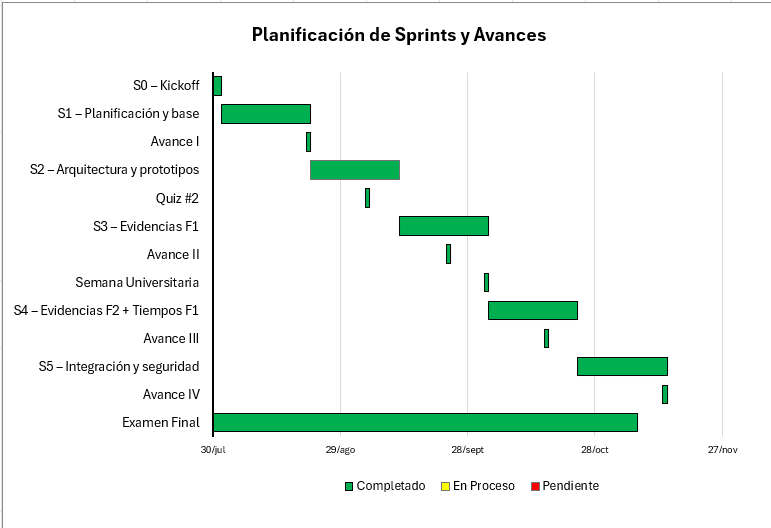
\includegraphics[width=\textwidth]{figs/cronograma (2).png}
    \caption{Cronograma de Sprints del Proyecto Ingeniería en Sistemas II.}
    \label{fig:cronograma-sprints}
\end{figure}
 % <<--- TODO el contenido de anexos vive aquí

% -------------------------------
% Bibliografía
% -------------------------------
\nocite{*}
\bibliographystyle{apalike}
\cleardoublepage
\phantomsection
\addcontentsline{toc}{chapter}{Referencias bibliográficas}
\bibliography{bib/ref}

\end{document}
